\documentclass[a4paper]{article}

\usepackage{marvosym}
\usepackage{url,parskip}			%formatting
\usepackage{tikz}
\usepackage{tkz-graph}
\usepackage{amsmath}

%better formatting of the A4 page
\usepackage{fullpage}
%An alternative to Layaureo can be usepackage{fullpage}
 
\usepackage{supertabular} 		%for Grades
\usepackage{titlesec}			%custom section

\usepackage{enumitem}
 
%Setup hyperref package, and colours for links
\usepackage{hyperref}

\begin{document}

\title{Graph Theory Assignment 1}
\author {
    Davies, Michael\\
    \and
    Goosen, Chris\\
    \and
    Laten, Matthew\\
    \and
    Sharwood, Bee\\
    \and
}
\maketitle

\subsection*{1.2 d)}
Firstly, we notice that to get from $Q_{t-1}$ to $Q_t$, we take the cartesian
product of $Q_{t-1}$ with $K_2$. This results in the number of vertices in
$Q_{t-1}$ being doubled. Since $Q_1 = K_1$ and the order of $Q_1$ is 2, we have
that the order of $Q_t$ is given by $2 \times 2 \times ... \times 2$ $t$ times,
or rather $ord(Q_t) = 2^t$.

To compute the size of $Q_t$, we interpret each vertex as a t-digit binary
string, which is adjacent to every binary string which differs from it by
exactly one place. Thus each vertex has degree $t$, the number of possible digits to vary.
Thus, the sum of the degrees of $Q_t$ is given by
\begin{equation}
    \sum_{v \in V(Q_t)} deg(v) = t\cdot2^t
\end{equation}
Thus, the size is $\frac{t\cdot2^t}{2} = t\cdot2^{t-1}$.

\subsection*{1.4}
We are looking for a graph which is cubic (3-regular) with order 7. However,
we know that the sum of the degrees for a graph has to be even. If such a graph
were to exist, the sum of the degrees would be $3 \times 7 = 21$ which is odd. 
Hence, no such graph exists.

\subsection*{1.5}
For a graph of degree $n$, the possible degrees a vertex in the graph can have
are $n-1, n-2, ..., 1, 0$. For an irregular such graph, each vertex must have
a distinct degree, and so each degree must be used exactly once. Thus, we get that
the vertex with degree $n-1$ must be adjacent to all other vertices, including
the vertex of degree $0$. The only situation where this is possible, is if
$n-1 = 0 \Rightarrow n = 1$ so there is only 1 vertex i.e. the graph is trivial.

\subsection*{1.6}

We start by noting that the possible handshake counts are 6, 5, 4, 3, 2, 1 and 0.
Each of these must be used once, and one number will be duplicated (my handshake count).


If we start by considering the order 6, we note that this person must shake hands with every
other guest (except his/her spouse). Then every other guest has degree $\geq 1$ and the only
candidate for 6's wife is 0. No other guest can shake 6 hands as they would need to shake hands
with 0, and no other guest can shake 0 hands as they have non-zero degree. We thus refer to these two people 
as ``6'' and ``0'' as they're definitely unique.

In the same spirit, we choose another random guest to have degree 5. This person has shaken hands
with 6, and cannot shake hands with 0 or his/her own spouse. Then he/she must connect to every person except 0.
Then, every person he/she shakes hands with must now have degree $\geq 2$. Then, the only candidate that could
possibly have degree 1 is 5's wife. No other guest can shake 5 hands as they would need to shake hands
with 0 or 1, then increasing these degrees, and no other guest can shake 1 hand as they have degree $\geq 2$. 
We thus refer to these two people as ``5'' and ``1'' as they're definitely unique.

We then choose a guest to have degree 4. This person cannot shake hands with 0, 1 or his/her own spouse. He/she
must then shake hands with 5, 6 and both remaining (as yet unnumbered) guests. This would increase those guests'
degrees by 1, so that they both have degree $geq 3$. The only guest left able to have degree 2 is 4's spouse.
Again, we know 4 is unique, as the not-yet-numbered vertices would need to shake hands with one of the already 
numbered vertices to increase their degree, which is not allowed, and they cannot shake hands with each other
as they are married.

Thus, the remaining two vertices both have degree 3.

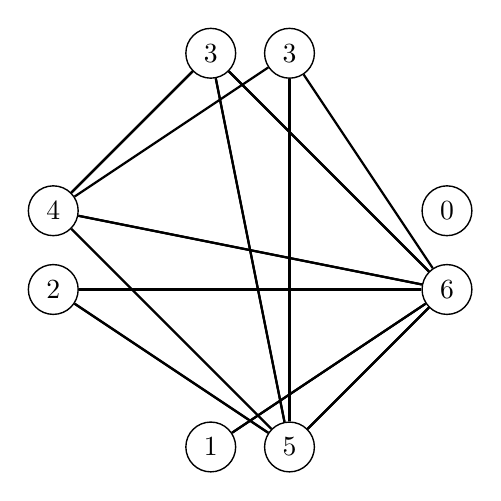
\begin{tikzpicture}
    \SetGraphUnit{2}
    \GraphInit[vstyle=Normal]
    \Vertex[x=0,y=2]{2}
    \Vertex[x=0,y=3]{4}
    \Vertex[x=2,y=0]{1}
    \Vertex[x=3,y=0]{5}
    \Vertex[x=5,y=2]{6}
    \Vertex[x=5,y=3]{0}
    \Vertex[x=2,y=5,L=3]{3A}
    \Vertex[x=3,y=5,L=3]{3B}
    \Edges(6, 1, 6, 2, 6, 4, 6, 5, 6, 3A, 6, 3B)
    \Edges(5, 2, 5, 3A, 5, 3B, 5, 4)
    \Edges(4, 3A, 4, 3B)
\end{tikzpicture}

\subsubsection*{1.6 a}
If I had a unique degree, then the answers I heard would have contained two 3s. Thus, I must be one of the 3s.
\subsubsection*{1.6 b}
Since we know the two 3s are married, my wife is the other 3.

\subsection*{1.7}
In order to prove this, we do a case distinction:\newline
\emph{Case r = 0:}

\subsection*{1.8}
\subsubsection*{a)} 
We need to show that if two graphs $G$ and $H$ are isomorphic, then they have the same degree sequence.
Let $f : V(G) \to V(H)$ be an isomorphism. We show that, for all $v \in V(G)$, $\mathrm{deg}_G(v) = \mathrm{deg}_H(f(v))$.

We have, for all $w \in V(H), v \in V(G)$,

\begin{align*}
w \in f(N(v)) &\Leftrightarrow f^{-1}(w)v \in E(G)\\
              &\Leftrightarrow wf(v) \in E(H)\\
              &\Leftrightarrow w \in N(f(v))
\end{align*}

Hence $f(N(v)) = N(f(v))$. Then

\begin{align*}
\mathrm{deg}_H(f(v)) &= |N(f(v))|\\
                     &= |f(N(v))|\\
                     &= |N(v)|\\
                     &= \mathrm{deg}_G(v)
\end{align*}

where the equation $|f(N(v))| = |N(v)|$ holds since $f$ is a bijection.

\subsubsection*{a)} 
This is false. A counterexample is:


\subsubsection*{a)}

\subsubsection*{b)}

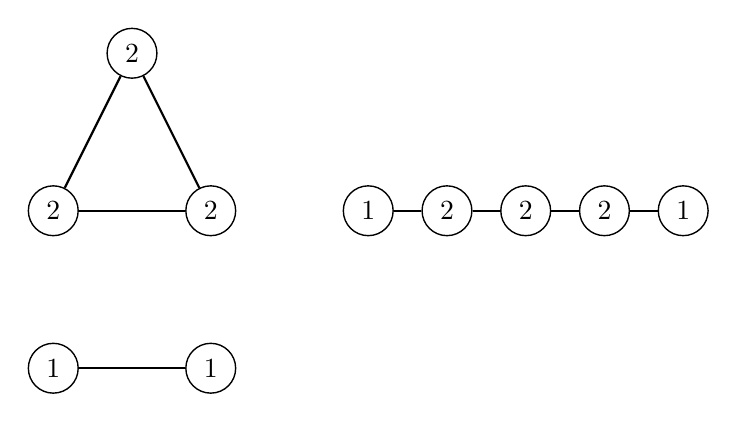
\begin{tikzpicture}
    \SetGraphUnit{2}
    \GraphInit[vstyle=Normal]
    \Vertex[x=0,y=2,L=2]{A}
    \Vertex[x=1,y=4,L=2]{B}
    \Vertex[x=2,y=2,L=2]{C}
    \Vertex[x=0,y=0,L=1]{D}
    \Vertex[x=2,y=0,L=1]{E}
    
    \Vertex[x=4,y=2,L=1]{F}
    \Vertex[x=5,y=2,L=2]{G}
    \Vertex[x=6,y=2,L=2]{H}
    \Vertex[x=7,y=2,L=2]{I}
    \Vertex[x=8,y=2,L=1]{J}
    
    \Edges(A, B, C, A)
    \Edge[](D)(E)
    \Edges(F, G, H, I, J)
\end{tikzpicture}


\subsection*{1.9 c)}

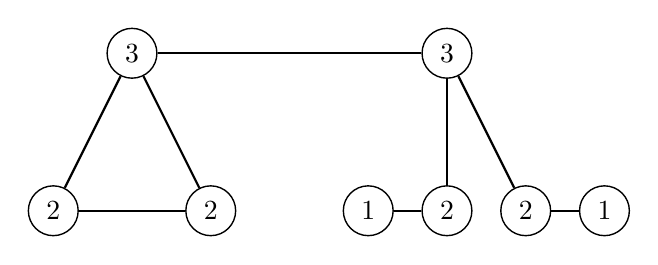
\begin{tikzpicture}
    \SetGraphUnit{2}
    \GraphInit[vstyle=Normal]
    \Vertex[x=0,y=0,L=2]{A}
    \Vertex[x=2,y=0,L=2]{B}
    \Vertex[x=1,y=2,L=3]{C}
    \Vertex[x=4,y=0,L=1]{D}
    \Vertex[x=5,y=0,L=2]{E}
    \Vertex[x=6,y=0,L=2]{F}
    \Vertex[x=7,y=0,L=1]{G}
    \Vertex[x=5,y=2,L=3]{H}
    \Edges(A, B, C, A)
    \Edges(C, H, E, D)
    \Edges(H, F, G)    
\end{tikzpicture}

\subsection*{1.9 d)}

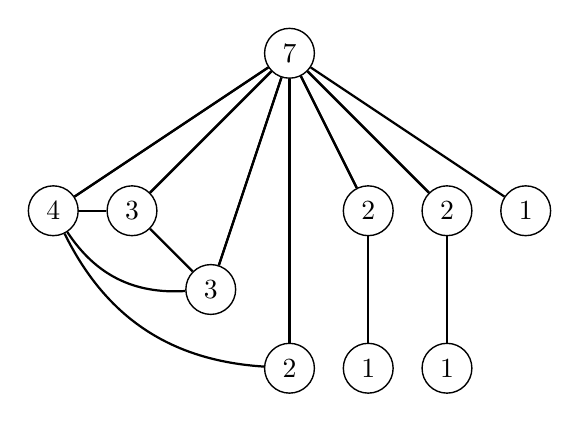
\begin{tikzpicture}
    \SetGraphUnit{2}
    \GraphInit[vstyle=Normal]
    \Vertex[x=3,y=4]{7}
    \Vertex[x=0,y=2]{4}
    \Vertex[x=1,y=2,L=3]{A}
    \Vertex[x=2,y=1,L=3]{B}
    \Vertex[x=3,y=0,L=2]{C}
    \Vertex[x=4,y=2,L=2]{D}
    \Vertex[x=5,y=2,L=2]{E}
    \Vertex[x=6,y=2,L=1]{F}
    \Vertex[x=4,y=0,L=1]{G}
    \Vertex[x=5,y=0,L=1]{H}
    \Edges(7, 4, 7, A, 7, B, 7, C, 7, D, 7, E, 7, F)
    \Edge[](4)(A)
    \Edge[style={bend right}](4)(B)
    \Edge[style={bend right}](4)(C)
    \Edge[](A)(B)
    \Edge[](D)(G)
    \Edge[](E)(H)    
\end{tikzpicture}

\subsection*{1.12} 

\subsection*{1.13}

\subsection*{1.15}

\subsubsection*{a)}

In the following images, $K_5$ is depicted with blue edges and $K_2$ is depicted with red edges. This is to improve the clarity of the images and make them more understandable. \\

$G + H$

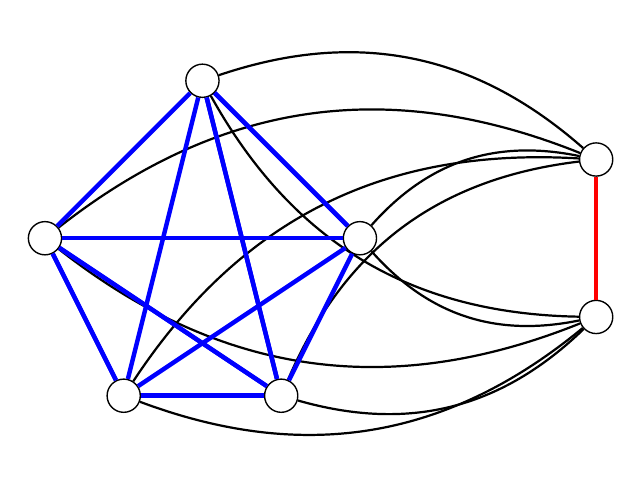
\begin{tikzpicture}
    \SetGraphUnit{2}
    \GraphInit[vstyle=Hasse]
    \Vertex[x=1,y=0]{A}
    \Vertex[x=0,y=2]{B}
    \Vertex[x=2,y=4]{C}
    \Vertex[x=3,y=0]{D}
    \Vertex[x=4,y=2]{E}
    
    \Vertex[x=7, y=3]{F}
    \Vertex[x=7, y=1]{G}
    
    \Edge[style={bend left}](A)(F)
    \Edge[style={bend right}](A)(G)
    
    \Edge[style={bend left}](B)(F)
    \Edge[style={bend right}](B)(G)
    
    \Edge[style={bend left}](C)(F)
    \Edge[style={bend right}](C)(G)
    
    \Edge[style={bend left}](D)(F)
    \Edge[style={bend right}](D)(G)
    
    \Edge[style={bend left}](E)(F)
    \Edge[style={bend right}](E)(G)
    
    \tikzset{EdgeStyle/.style = {ultra thick, color = blue}}
    \Edges(A, B, C, D, E, A, C, D, A, B, D, B, E, C, E)

    \tikzset{EdgeStyle/.style = {ultra thick, color = red}}
    \Edge[](F)(G)
     
\end{tikzpicture}

$G \times H$

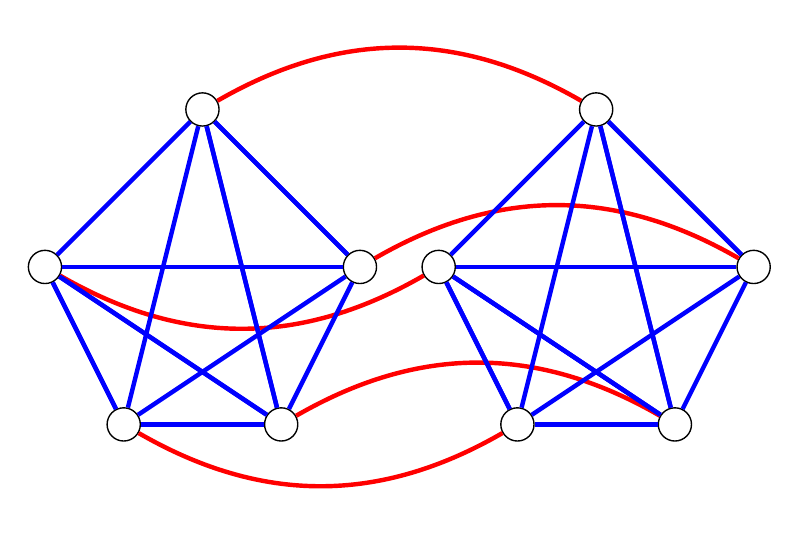
\begin{tikzpicture}
    \SetGraphUnit{2}
    \GraphInit[vstyle=Hasse]
    \Vertex[x=1,y=0]{A}
    \Vertex[x=0,y=2]{B}
    \Vertex[x=2,y=4]{C}
    \Vertex[x=3,y=0]{D}
    \Vertex[x=4,y=2]{E}
    
    \Vertex[x=6,y=0]{1A}
    \Vertex[x=5,y=2]{1B}
    \Vertex[x=7,y=4]{1C}
    \Vertex[x=8,y=0]{1D}
    \Vertex[x=9,y=2]{1E}
    
    \tikzset{EdgeStyle/.style = {ultra thick, color = red}}
    \Edge[style={bend right}](A)(1A)
    \Edge[style={bend right}](B)(1B)
    \Edge[style={bend left}](C)(1C)
    \Edge[style={bend left}](D)(1D)
    \Edge[style={bend left}](E)(1E)
   
    \tikzset{EdgeStyle/.style = {ultra thick, color = blue}}
    \Edges(A, B, C, D, E, A, C, D, A, B, D, B, E, C, E)
    \Edges(1A, 1B, 1C, 1D, 1E, 1A, 1C, 1D, 1A, 1B, 1D, 1B, 1E, 1C, 1E) 
\end{tikzpicture}

\subsubsection*{b)}

$\overline{K}_5 + \overline{K}_3$

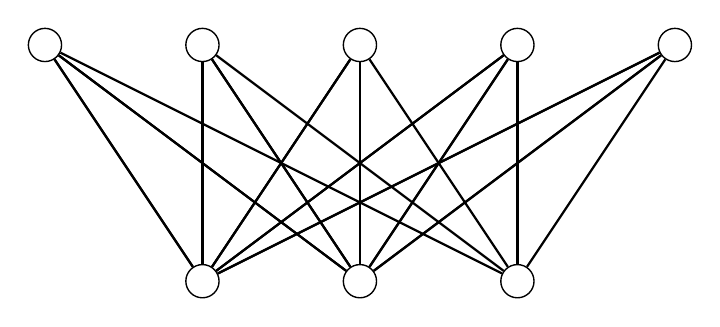
\begin{tikzpicture}

    \SetGraphUnit{2}
    \GraphInit[vstyle=Hasse]
    \Vertex[x=0,y=3]{A}
    \Vertex[x=2,y=3]{B}
    \Vertex[x=4,y=3]{C}
    \Vertex[x=6,y=3]{D}
    \Vertex[x=8,y=3]{E}
    
    \Vertex[x=2,y=0]{F}
    \Vertex[x=4,y=0]{G}
    \Vertex[x=6,y=0]{H}
    
    \Edges(A, F, A, G, A, H)
    \Edges(B, F, B, G, B, H)  
    \Edges(C, F, C, G, C, H)
    \Edges(D, F, D, G, D, H)
    \Edges(E, F, E, G, E, H)

\end{tikzpicture}

$\overline{K}_5 \times \overline{K}_3$

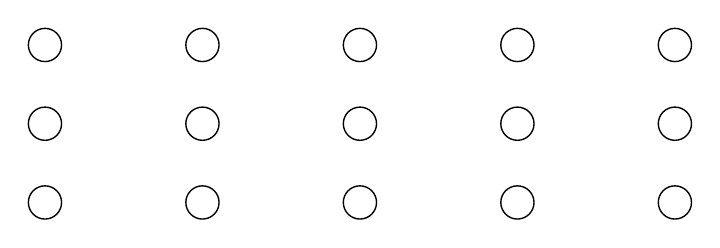
\begin{tikzpicture}
    \SetGraphUnit{2}
    \GraphInit[vstyle=Hasse]
    \Vertex[x=0,y=3]{A}
    \Vertex[x=2,y=3]{B}
    \Vertex[x=4,y=3]{C}
    \Vertex[x=6,y=3]{D}
    \Vertex[x=8,y=3]{E}
    
    \Vertex[x=0,y=2]{1A}
    \Vertex[x=2,y=2]{1B}
    \Vertex[x=4,y=2]{1C}
    \Vertex[x=6,y=2]{1D}
    \Vertex[x=8,y=2]{1E}
    
    \Vertex[x=0,y=1]{2A}
    \Vertex[x=2,y=1]{2B}
    \Vertex[x=4,y=1]{2C}
    \Vertex[x=6,y=1]{2D}
    \Vertex[x=8,y=1]{2E}
\end{tikzpicture}

\subsubsection*{c)}

In the following graphs, the edges of $C_5$ are coloured blue for clarity. \\

$C_5 + K_1$

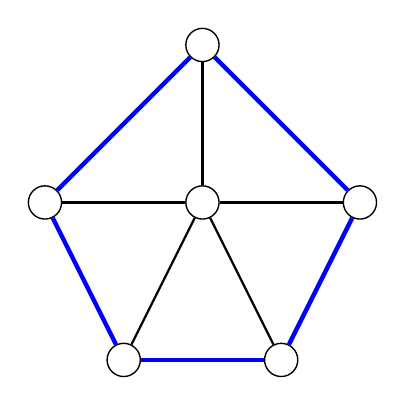
\begin{tikzpicture}
    \SetGraphUnit{2}
    \GraphInit[vstyle=Hasse]
    \Vertex[x=1,y=0]{A}
    \Vertex[x=0,y=2]{B}
    \Vertex[x=2,y=4]{C}
    \Vertex[x=3,y=0]{D}
    \Vertex[x=4,y=2]{E}
    
    \Vertex[x=2,y=2]{F}

    \Edge[](A)(F)
    \Edge[](B)(F)
    \Edge[](C)(F)
    \Edge[](D)(F)
    \Edge[](E)(F)
    
    \tikzset{EdgeStyle/.style = {ultra thick, color = blue}}
    \Edges(A,B,C,E,D,A)
\end{tikzpicture}

$C_5 \times K_1$

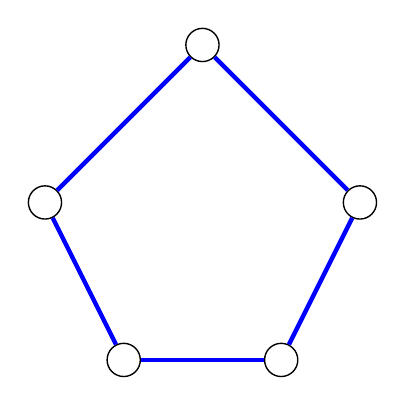
\begin{tikzpicture}
    \SetGraphUnit{2}
    \GraphInit[vstyle=Hasse]
    \Vertex[x=1,y=0]{A}
    \Vertex[x=0,y=2]{B}
    \Vertex[x=2,y=4]{C}
    \Vertex[x=3,y=0]{D}
    \Vertex[x=4,y=2]{E}
    
    \tikzset{EdgeStyle/.style = {ultra thick, color = blue}}
    \Edges(A,B,C,E,D,A)
\end{tikzpicture}

\subsection*{1.16}

\subsubsection*{$G_0$}

\begin{tikzpicture}
    \SetGraphUnit{2}
    \GraphInit[vstyle=Hasse]
    \Vertex[x=3,y=1]{iA}
    \Vertex[x=2,y=3]{iB}
    \Vertex[x=4,y=5]{iC}
    \Vertex[x=6,y=3]{iD}
    \Vertex[x=5,y=1]{iE}  
    
    \Vertex[x=2,y=0]{oA}
    \Vertex[x=1,y=3]{oB}
    \Vertex[x=4,y=6]{oC}
    \Vertex[x=7,y=3]{oD}
    \Vertex[x=6,y=0]{oE}  
\end{tikzpicture}

\subsubsection*{$G_1$}

\begin{tikzpicture}
    \SetGraphUnit{2}
    \GraphInit[vstyle=Hasse]
    \Vertex[x=3,y=1]{iA}
    \Vertex[x=2,y=3]{iB}
    \Vertex[x=4,y=5]{iC}
    \Vertex[x=6,y=3]{iD}
    \Vertex[x=5,y=1]{iE}  
    
    \Vertex[x=2,y=0]{oA}
    \Vertex[x=1,y=3]{oB}
    \Vertex[x=4,y=6]{oC}
    \Vertex[x=7,y=3]{oD}
    \Vertex[x=6,y=0]{oE}  
    
    \Edge[](iA)(oA)
    \Edge[](iB)(oB)
    \Edge[](iC)(oC)
    \Edge[](iD)(oD)
    \Edge[](iE)(oE)
\end{tikzpicture}

\subsubsection*{$G_2$}

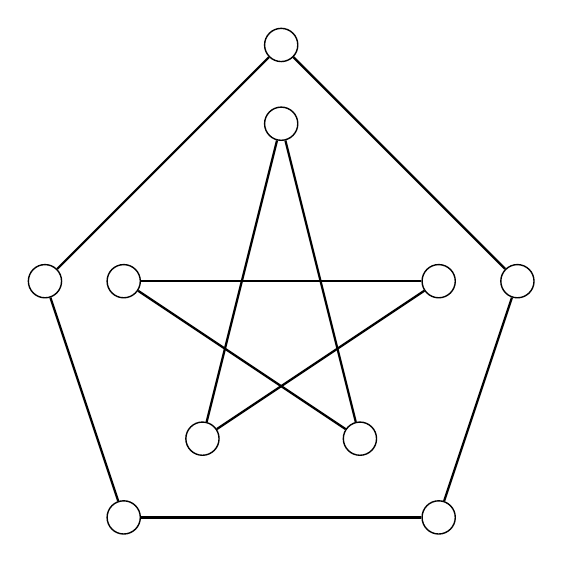
\begin{tikzpicture}
    \SetGraphUnit{2}
    \GraphInit[vstyle=Hasse]
    \Vertex[x=3,y=1]{iA}
    \Vertex[x=2,y=3]{iB}
    \Vertex[x=4,y=5]{iC}
    \Vertex[x=6,y=3]{iD}
    \Vertex[x=5,y=1]{iE}  
    
    \Vertex[x=2,y=0]{oA}
    \Vertex[x=1,y=3]{oB}
    \Vertex[x=4,y=6]{oC}
    \Vertex[x=7,y=3]{oD}
    \Vertex[x=6,y=0]{oE}  
    
    \Edges(oA, oB, oC, oD, oE, oA)
    \Edges(iA, iC, iE, iB, iD, iA)
\end{tikzpicture}

\subsubsection*{$G_3$}

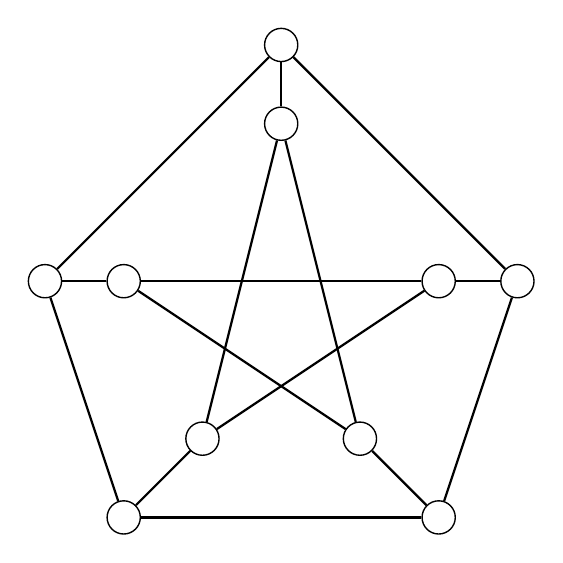
\begin{tikzpicture}
    \SetGraphUnit{2}
    \GraphInit[vstyle=Hasse]
    \Vertex[x=3,y=1]{iA}
    \Vertex[x=2,y=3]{iB}
    \Vertex[x=4,y=5]{iC}
    \Vertex[x=6,y=3]{iD}
    \Vertex[x=5,y=1]{iE}  
    
    \Vertex[x=2,y=0]{oA}
    \Vertex[x=1,y=3]{oB}
    \Vertex[x=4,y=6]{oC}
    \Vertex[x=7,y=3]{oD}
    \Vertex[x=6,y=0]{oE}  
    
    \Edges(oA, oB, oC, oD, oE, oA)
    \Edges(iA, iC, iE, iB, iD, iA)
    
    \Edge[](iA)(oA)
    \Edge[](iB)(oB)
    \Edge[](iC)(oC)
    \Edge[](iD)(oD)
    \Edge[](iE)(oE)
\end{tikzpicture}

\subsection*{1.17}
If $G$ and $\bar G$ are both $r$-regular where $r \geq 0$, we want to
show that the order of $G$ is odd.  First we notice that
\begin{equation} 
    \sum_{v \in V(G)} deg_G(v) = n \cdot r = 2m   
\end{equation}
Next we see that
\begin{equation} 
    \sum_{v \in V(\bar G)} deg_{\bar G}(v) = n \cdot r = 2m   
\end{equation}
However
\begin{eqnarray*} 
    &\sum_{v \in V(\bar G)} ((n-1) - deg_G(V))\\
    &n(n-1) - nr = nr\\
    &\Rightarrow n(n-1) = 2nr\\
    &\Rightarrow n-1 = 2r\\
    &\Rightarrow n-1\ is\ even\\
    &\Rightarrow n\ is\ odd\\
\end{eqnarray*}




\subsection*{1.18 b)}
If $G$ is a self-complementary graph of order $n$, this means that $G \cup \bar G = K_n$.
Thus, $size(G) = \frac{1}{2} size(K_n) = \frac{1}{4}n(n-1)$.

\subsection*{1.19}

\subsubsection*{a)}

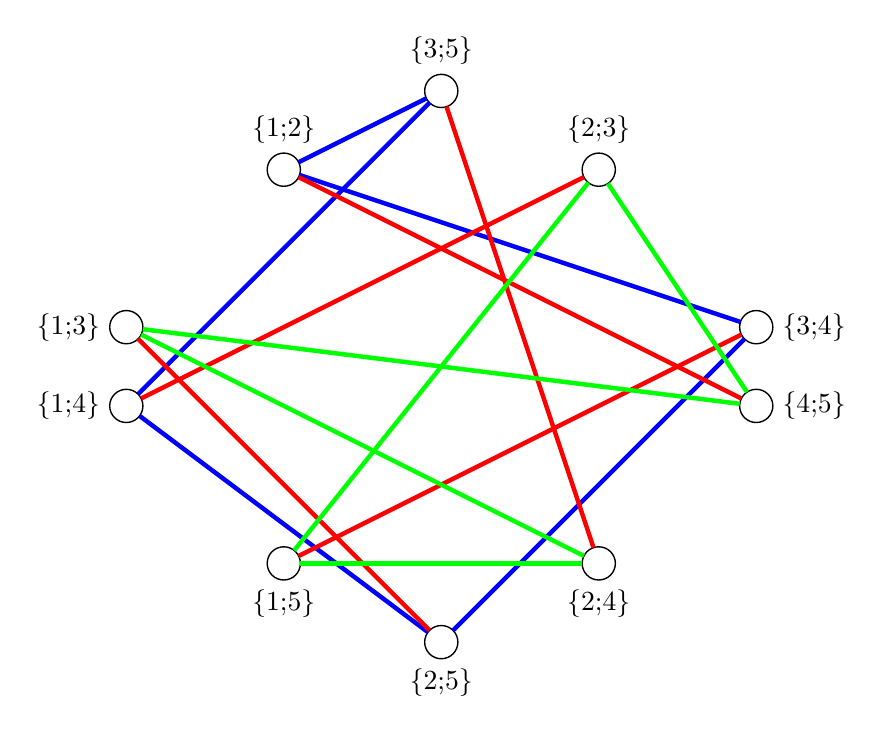
\begin{tikzpicture}
    \SetGraphUnit{2}
    \GraphInit[vstyle=Welsh]
    \Vertex[x=0,y=4,L=\{1;4\},Lpos=180]{A}
    \Vertex[x=0,y=5,L=\{1;3\},Lpos=180]{B}
    \Vertex[x=2,y=7,L=\{1;2\},Lpos=90]{C}
    \Vertex[x=4,y=8,L=\{3;5\},Lpos=90]{D}
    \Vertex[x=6,y=7,L=\{2;3\},Lpos=90]{E}
    \Vertex[x=8,y=5,L=\{3;4\}]{F}
    \Vertex[x=8,y=4,L=\{4;5\}]{G}
    \Vertex[x=6,y=2,L=\{2;4\},Lpos=270]{H}
    \Vertex[x=4,y=1,L=\{2;5\},Lpos=270]{I}
    \Vertex[x=2,y=2,L=\{1;5\},Lpos=270]{J}  
  
    \tikzset{EdgeStyle/.style = {ultra thick, color = blue}}
    \Edge[](A)(D)
    \Edge[](A)(I)
    \Edge[](C)(D)
    \Edge[](C)(F)
    \Edge[](F)(I)
    
    \tikzset{EdgeStyle/.style = {ultra thick, color = red}}
    \Edge[](A)(E)
    \Edge[](F)(J)
    \Edge[](D)(H)
    \Edge[](C)(G)
    \Edge[](B)(I)
    
    \tikzset{EdgeStyle/.style = {ultra thick, color = green}}
    \Edge[](B)(H)
    \Edge[](B)(G)
    \Edge[](E)(G)
    \Edge[](E)(J)
    \Edge[](H)(J)
\end{tikzpicture}

\subsubsection*{b)}

Because $k$-subsets of $n$ exist the order of $J(n,k,r)$ is 

\begin{equation}
n \choose k
\end{equation}

\subsubsection*{c)}

For a given vertex, we first choose $r$ elements which it will have in common and then, from the remaining elements choose $(k-r)$ extra elements to find a vertex which is adjacent to it. Each of these will be a unique choice. Thus each vertex has degree

\begin{equation}
    \mathrm{deg}(v) = {k \choose r} {n-k \choose k-r}
\end{equation}

and thus the graph is regular. The size of the graph is

\begin{equation}
n {k \choose r} {n-k \choose k-r}
\end{equation}

\subsubsection*{d)}

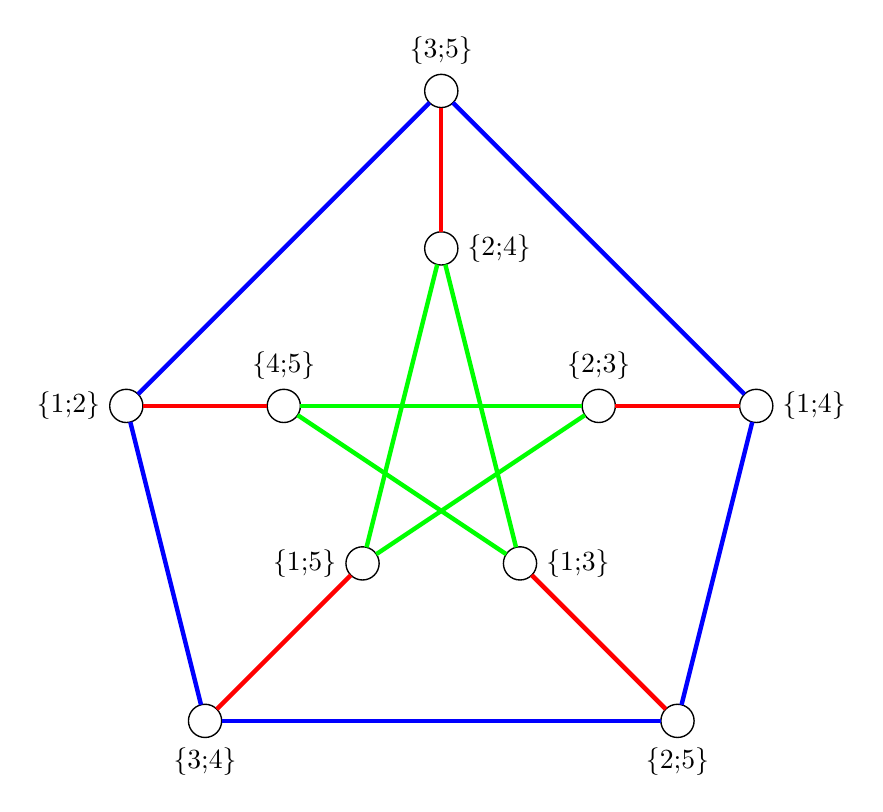
\begin{tikzpicture}
    \SetGraphUnit{2}
    \GraphInit[vstyle=Welsh]
    \Vertex[x=3,y=1,L=\{1;5\},Lpos=180]{iA}
    \Vertex[x=2,y=3,L=\{4;5\},Lpos=90]{iB}
    \Vertex[x=4,y=5,L=\{2;4\}]{iC}
    \Vertex[x=6,y=3,L=\{2;3\},Lpos=90]{iD}
    \Vertex[x=5,y=1,L=\{1;3\}]{iE}  
    
    \Vertex[x=1,y=-1,L=\{3;4\},Lpos=270]{oA}
    \Vertex[x=0,y=3,L=\{1;2\},Lpos=180]{oB}
    \Vertex[x=4,y=7,L=\{3;5\},Lpos=90]{oC}
    \Vertex[x=8,y=3,L=\{1;4\}]{oD}
    \Vertex[x=7,y=-1,L=\{2;5\},Lpos=270]{oE}  
    
    \tikzset{EdgeStyle/.style = {ultra thick, color = blue}}
    \Edges(oA, oB, oC, oD, oE, oA)
    
    \tikzset{EdgeStyle/.style = {ultra thick, color = green}}
    \Edges(iA, iC, iE, iB, iD, iA)
    
    \tikzset{EdgeStyle/.style = {ultra thick, color = red}}
    \Edge[](iA)(oA)
    \Edge[](iB)(oB)
    \Edge[](iC)(oC)
    \Edge[](iD)(oD)
    \Edge[](iE)(oE)
\end{tikzpicture}

\end{document}
